\documentclass[11pt]{article}
\usepackage[utf8]{inputenc}
\usepackage[margin=1in]{geometry}
\usepackage{amsmath,amssymb,amsfonts}
\usepackage{graphicx}
\usepackage{booktabs}
\usepackage{hyperref}
\usepackage{algorithm}
\usepackage{algorithmic}
\usepackage{multirow}
\usepackage{natbib}
\usepackage{setspace}
\usepackage{caption}
\usepackage{subcaption}
\usepackage{float}
\usepackage{enumitem}
\usepackage{xcolor}

\hypersetup{
    colorlinks=true,
    linkcolor=blue!70!black,
    citecolor=blue!70!black,
    urlcolor=blue!70!black,
}

\onehalfspacing

% Figures are in paper/fig/ or output/figures/
\graphicspath{{fig/}{paper/fig/}{../output/figures/}{output/figures/}}

\title{\textbf{Multi-Scale Regime Detection with Fuzzy Aggregation\\for Adaptive Sector Portfolio Management}}

\author{
Tanishk Yadav\thanks{ORCID: 0009-0006-2382-9411.}\\
\textit{MS Financial Engineering}\\
NYU Tandon School of Engineering\\
New York, NY, USA
}

\date{}

\begin{document}

\maketitle

% ─── ABSTRACT ────────────────────────────────────────────────────────────────
\begin{abstract}
\noindent
We propose a multi-scale regime detection framework that fuses four
\emph{orthogonal} stress detectors---CUSUM sequential analysis on
z-score returns (magnitude), rolling cross-sector correlation
(structure / contagion), market breadth (participation), and rolling
return skewness (left-tail asymmetry)---into a unified stress
probability via sigmoid-membership fuzzy inference. Crucially, the
aggregator uses a \emph{max-of-top-2} rule: it returns the
second-largest membership, so at least two orthogonal detectors must
agree before the system acts, structurally suppressing single-detector
false alarms. The composite signal drives an adaptive sector portfolio
that classifies eleven S\&P~500 sector ETFs into three baskets
(Tactical, Avoid, Core) by GARCH(1,1)-$t$ conditional-volatility
terciles and Ornstein-Uhlenbeck recovery half-life, with implicit cash
allocation as the primary risk-reduction mechanism. In a walk-forward
backtest (2009--2025, quarterly recalibration, 10 bps/trade, zero
look-ahead), the framework is best understood as a
\emph{capital-preservation overlay}: it holds maximum drawdown to
$-6.2\%$ (versus $-41.7\%$ for SPY) at $4.6\%$ annualized volatility,
for a Sharpe of $0.97$ (versus SPY's $0.58$) and Calmar $0.94$.
Benchmarked honestly, simple trend rules achieve higher \emph{raw}
Sharpe on the SPY universe; the architecture's distinctive value is
\emph{generalization}---applied unchanged to factor portfolios and
international equities it scores Sharpe $1.21$ and $1.04$ against
$0.51$ and $0.11$ for equal-weight, where a single index-tuned rule
would not transfer. All parameters are estimated from data with zero
look-ahead bias enforced throughout.

\medskip
\noindent\textbf{Keywords:} regime detection, fuzzy consensus, portfolio management, capital preservation, CUSUM, cross-asset generalization, GARCH, walk-forward validation, implicit cash allocation
\end{abstract}

% ─── INTRODUCTION ────────────────────────────────────────────────────────────
\section{Introduction}

Financial markets exhibit regime-dependent behavior characterized by
distinct periods of calm, transition, and stress
\citep{hamilton1989}.  Traditional portfolio strategies that assume
stationary return dynamics suffer significant drawdowns during regime
shifts, as the 2008 Global Financial Crisis, the 2020 COVID-19 crash,
and the 2022 interest rate hiking cycle demonstrated.  Even
diversified portfolios that hold all sectors with equal or
risk-proportional weights cannot avoid the synchronous drawdowns
that characterize systemic stress events.

The central challenge in regime-adaptive portfolio management is
\emph{timely} and \emph{reliable} regime detection.  Individual
detectors operate on different time-scales and suffer from distinct
failure modes: short-term indicators produce false alarms during
idiosyncratic volatility, while long-term models react too slowly to
protect against rapid drawdowns.  The secondary challenge is
translating regime signals into portfolio actions that actually reduce
risk: a system that detects stress but merely redistributes weight
among risky assets---rather than moving to cash---provides limited
drawdown protection.

This paper addresses both challenges.  We propose an ensemble
architecture that fuses four \emph{orthogonal} stress detectors through
a weightless fuzzy consensus rule, combined with an adaptive basket
allocation framework where implicit cash allocation serves as the
primary risk-reduction mechanism.

Our contributions are fourfold:
\begin{enumerate}[itemsep=2pt]
    \item A four-detector ensemble spanning complementary, orthogonal
          dimensions of stress---CUSUM on z-score-standardized returns
          (magnitude, scale-invariant), cross-sector correlation
          (structure), market breadth (participation), and rolling
          return skewness (left-tail asymmetry, leading).
    \item A \emph{weightless} fuzzy aggregator: per-detector sigmoid
          memberships are Brier-calibrated against realized drawdowns,
          and the composite is the second-largest membership (a
          max-of-top-2, 2-of-4 consensus). No single detector can act
          alone, structurally suppressing false alarms with no detector
          weights to over-fit.
    \item A tercile-based basket construction that classifies sector
          ETFs using GARCH(1,1)-$t$ conditional volatility and
          Ornstein-Uhlenbeck recovery dynamics, with graduated
          Core-basket response to extreme stress.
    \item An implicit cash mechanism where stress-induced weight
          reduction produces sub-unity portfolio allocation, the
          deficit earning the risk-free rate rather than being
          redistributed to other risky assets.
\end{enumerate}

% ─── RELATED WORK ────────────────────────────────────────────────────────────
\section{Related Work}

\citet{hamilton1989} introduced Markov-switching models for business
cycle analysis, establishing the foundation for regime-based asset
allocation.  \citet{ang2002} extended this framework to international
asset allocation, demonstrating that regime-switching models can
improve out-of-sample portfolio performance when properly calibrated.
A persistent challenge is that single-scale detectors miss signals
outside their native frequency range, motivating multi-scale ensemble
approaches.

\citet{gradojevic2013} demonstrated the effectiveness of fuzzy logic
systems for financial decision-making under uncertainty.  The
sigmoid-membership fuzzy framework \citep{takagi1985} provides a
principled approach to combining multiple information sources with
calibratable membership functions.  Our work adapts this with a
\emph{weightless} max-of-top-2 consensus---calibrating only membership
shape parameters, with no detector weights---to
prevent degenerate solutions.

\citet{nystrup2017} showed that regime-based asset allocation
outperforms static strategies when the regime model is properly
calibrated.  \citet{kirby2012} demonstrated that simple timing
strategies based on inverse-volatility weighting outperform na\"ive
diversification.  Our framework builds on inverse-volatility weighting
as the base allocation and adds regime-dependent scaling with an
implicit cash buffer.

\citet{page1954} introduced the CUSUM procedure for sequential change
detection.  \citet{killick2012} proposed the PELT algorithm for
optimal change-point detection with linear computational cost.
\citet{siegmund1985} derived ARL approximations for setting CUSUM
decision thresholds.  We apply CUSUM to z-score-standardized returns
to achieve scale-invariant detection thresholds.

% ─── ARCHITECTURE ────────────────────────────────────────────────────────────
\section{System Architecture}

Figure~\ref{fig:architecture} presents the complete system architecture.
The framework operates in four layers: data acquisition, multi-scale
detection with fuzzy aggregation, asset characterization and
classification, and adaptive portfolio construction with implicit cash
allocation.  All parameters are re-estimated at each quarterly
walk-forward step using only past data, ensuring zero lookahead bias.

\begin{figure}[H]
\centering
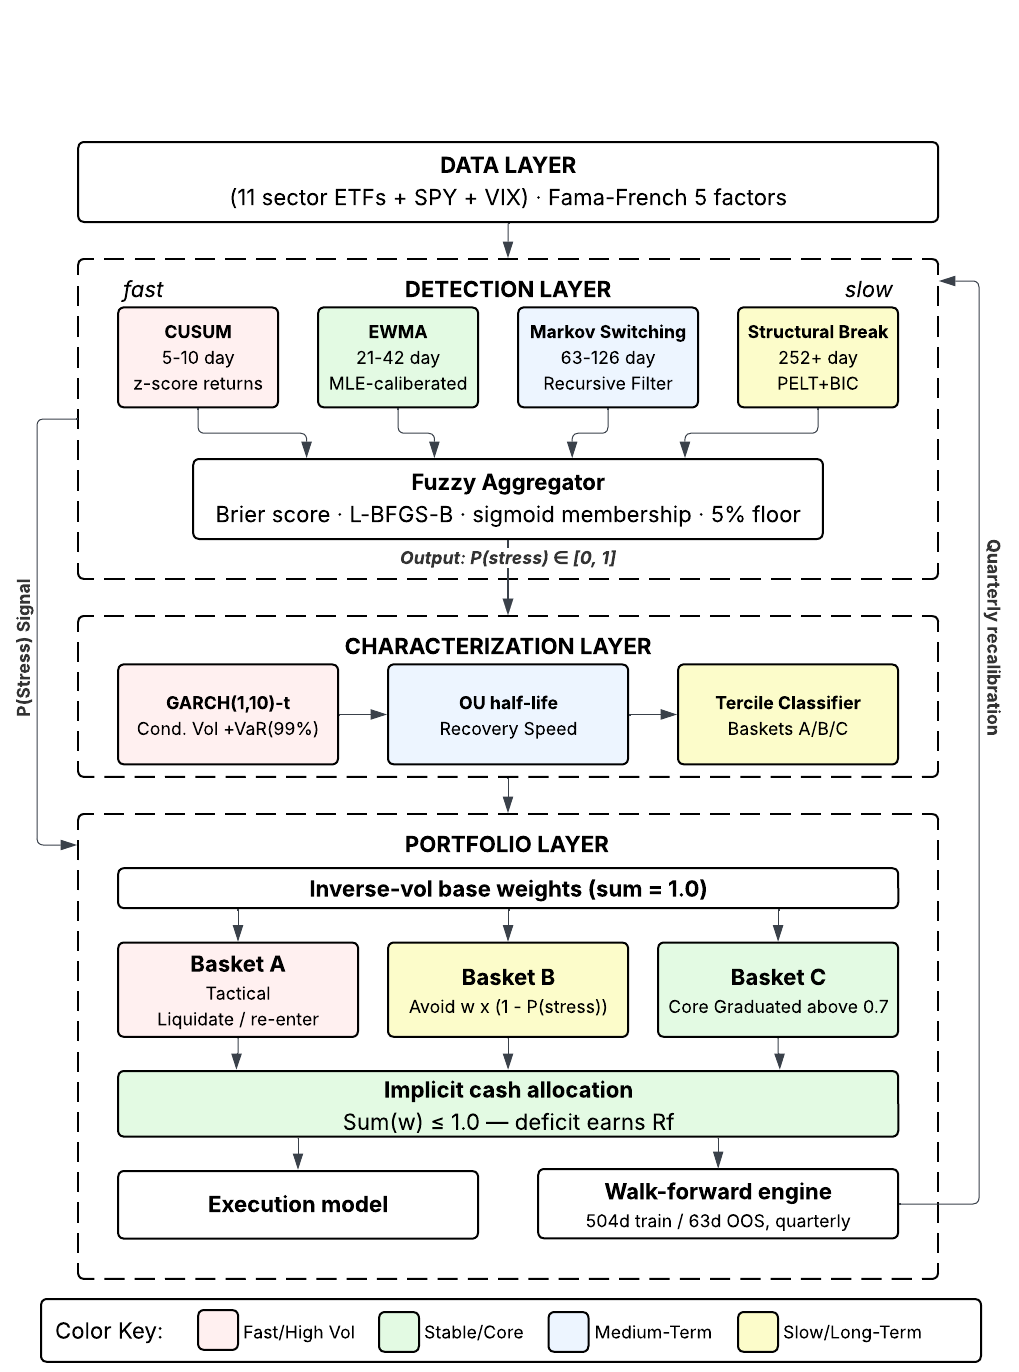
\includegraphics[width=\textwidth]{architecture.png}
\caption{System architecture.  Four detectors spanning 5-day to
252+-day horizons feed into a Brier-score-optimized fuzzy aggregator.
The composite stress probability drives adaptive basket allocation
with implicit cash as the risk-reduction mechanism.  All parameters
are re-estimated at each walk-forward step.}
\label{fig:architecture}
\end{figure}

% ─── METHODOLOGY ─────────────────────────────────────────────────────────────
\section{Methodology}

\subsection{Multi-Scale Detector Ensemble}

We deploy four detectors targeting complementary time-scales.  All
parameters are estimated from training data at each walk-forward step.
Figure~\ref{fig:regime} illustrates the coordinated response of all
four detectors over the full out-of-sample period, demonstrating how
their complementary time-scales capture different aspects of market
stress.

\subsubsection{CUSUM Sequential Detector (5--10 day)}
Following \citet{page1954}, we maintain upward and downward CUSUM
accumulators on \emph{z-score-standardized} returns:
\begin{equation}
    z_t = \frac{r_t - \hat{\mu}_0}{\hat{\sigma}_{\text{train}}}
\end{equation}
\begin{align}
    S_t^+ &= \max(0,\; S_{t-1}^+ + z_t - k) \\
    S_t^- &= \max(0,\; S_{t-1}^- - z_t - k)
\end{align}
where $\hat{\mu}_0$ and $\hat{\sigma}_{\text{train}}$ are the mean and
standard deviation of training-window returns, $k = 0.5$ (detecting a
1$\sigma$ shift in standardized space), and the decision threshold is
$h = (\ln(\text{ARL}_0) + 1.166) / \delta$ with $\delta = 1$ per
\citet{siegmund1985}, yielding $h \approx 6.70$ for a target average
run length of 252 trading days.  The signal is
$\min(\max(S_t^+, S_t^-)/h,\; 1)$.

Operating in z-score space makes the threshold \emph{scale-invariant}: a
single $-5\%$ daily return (approximately $z = -4.2$) produces a signal
of $\sim\!0.55$, while three consecutive $-2\%$ days ($z \approx -1.7$
each) yield a signal of $\sim\!0.54$.  Under the original raw-return
formulation, the threshold was approximately 558, requiring over
12{,}000 consecutive crash days to trigger---rendering the detector
inoperative.

\subsubsection{Cross-Sector Correlation (21-day)}
We compute the average pairwise Pearson correlation across the eleven
sector ETFs over a rolling 21-day window. Rising average correlation
signals diversification collapse and contagion---a dimension of stress
distinct in kind from return magnitude. The raw correlation is mapped
linearly from $[0.10, 0.60]$ to $[0,1]$ and clipped. This detector also
serves as a structural-break proxy: when its signal exceeds $0.5$,
Basket~C (core holdings) is zeroed.

\subsubsection{Market Breadth (21-day)}
Breadth measures \emph{participation}: the fraction of the eleven
sectors with negative cumulative returns over a rolling 21-day window,
mapped linearly from $[0.05, 0.50]$ to $[0,1]$. It is orthogonal to
CUSUM because it captures \emph{how many} sectors are declining, not
how far any single one has moved---broad, shallow weakness scores high
here while one violent sector move does not.

\subsubsection{Return Skewness (63-day)}
We compute the 63-day rolling Fisher skewness of benchmark (SPY)
returns, mapped from $[-0.8, 0]$ to $[1, 0]$ so that strongly negative
skew yields a high signal. Left-tail fattening frequently precedes
realized drawdowns, making this the ensemble's leading-indicator
dimension. Like the other detectors, its mapping bounds are fixed a
priori; no parameter is tuned on test data.

\subsection{Fuzzy Aggregation Framework}

Each detector signal $x_i \in [0,1]$ passes through a calibrated
sigmoid membership function:
\begin{equation}
    \mu_i(x_i) = \frac{1}{1 + \exp(-a_i(x_i - c_i))}
\end{equation}
where $a_i$ (steepness) and $c_i$ (crossover point) are per-detector
parameters. Rather than a weighted sum, the composite stress
probability is the \emph{second-largest} membership---a max-of-top-2,
or 2-of-4 consensus, rule:
\begin{equation}
    P(\text{stress}) = \mu_{(2)}, \qquad
    \mu_{(1)} \ge \mu_{(2)} \ge \mu_{(3)} \ge \mu_{(4)} .
\end{equation}
This requires at least two of the four orthogonal detectors to show
elevated stress before the system acts: a single detector firing---a
likely false alarm---leaves the second-largest membership low. The
design is deliberately \emph{weightless}; there are no detector weights
to over-fit, only the sigmoid shape parameters are learned, and no
single detector can move the portfolio on its own.

The sigmoid parameters $\{a_i, c_i\}$ are calibrated by minimizing the
Brier score \citep{brier1950} against realized drawdowns in the
training window:
\begin{equation}
    \mathcal{L}_{\text{Brier}} = \frac{1}{T}\sum_{t=1}^{T}
    \bigl(P_{\text{stress},t} - D_t\bigr)^2
\end{equation}
where $D_t = 1$ if a drawdown exceeding the 10th percentile of
training-window drawdowns occurs within the next 21 trading days.
Optimization uses L-BFGS-B with bounds $a_i \in [1, 50]$ and
$c_i \in [0.05, 0.95]$.

\begin{figure}[H]
\centering

\includegraphics[width=\textwidth]{membership_functions.png}
\caption{Calibrated sigmoid membership functions for each detector. The
crossover point $c$ (dashed line) marks where stress membership equals
0.5. The composite stress signal is the \emph{second-largest} of the
four memberships (2-of-4 consensus), so at least two orthogonal
detectors must agree before the system de-risks.}
\label{fig:membership}
\end{figure}

\subsection{Asset Characterization}

\subsubsection{GARCH(1,1)-$t$ Conditional Volatility}
For each sector ETF, we estimate \citep{bollerslev1986, engle1982}:
\begin{equation}
    \sigma_t^2 = \omega + \alpha\varepsilon_{t-1}^2
               + \beta\sigma_{t-1}^2, \quad
    z_t \sim t_\nu
\end{equation}
yielding conditional VaR(99\%) =
$\hat{\mu} + \hat{\sigma}_t \cdot t_\nu^{-1}(0.01) \cdot
\sqrt{(\nu-2)/\nu}$.

\subsubsection{Ornstein-Uhlenbeck Recovery Half-Life}
We model drawdown recovery as a discretized OU
process \citep{uhlenbeck1930}:
\begin{equation}
    \Delta X_t = \kappa(\theta - X_{t-1})\Delta t + \varepsilon_t
\end{equation}
The half-life $\ln(2)/\kappa$ measures recovery speed.  Sectors with
$\kappa \leq 0$ are flagged as non-mean-reverting.

\subsection{Adaptive Basket Construction}

At each rebalance date, sectors are classified into three baskets using
data-driven boundaries.  We use \emph{tercile} boundaries on
conditional volatility (33rd and 67th percentiles of the
cross-sectional vol distribution) combined with median half-life:

\begin{itemize}[itemsep=4pt]
    \item \textbf{Basket~A (Tactical):} Top or middle tercile vol with
          fast recovery ($\text{HL} < \text{median}$).  Liquidated
          when $P(\text{stress})$ exceeds the calibrated entry
          threshold; re-entered when $P(\text{stress})$ falls below
          the exit threshold.
    \item \textbf{Basket~B (Avoid):} Top tercile vol with slow
          recovery ($\text{HL} \geq \text{median}$).  Continuously
          de-risked: $w_i = w_i^{\text{base}} \cdot
          (1 - P(\text{stress}))$.
    \item \textbf{Basket~C (Core):} Bottom tercile vol.  Held at
          full weight through mild stress.  Above
          $P(\text{stress}) = 0.7$, graduated linear scaling:
          \begin{equation}
              w_i = w_i^{\text{base}} \cdot
              \max\!\left(0,\;
              \frac{1 - P(\text{stress})}{0.3}\right)
          \end{equation}
          This preserves stability during moderate corrections while
          enabling full de-risking during tail events.
\end{itemize}

Figure~\ref{fig:scatter} shows the resulting classification landscape.
Energy (XLE), with high conditional VaR and fast recovery, is
classified as Tactical (Basket~A).  Financials (XLF) and Consumer
Discretionary (XLY), with high VaR but slower recovery, fall into
Avoid (Basket~B).  The remaining sectors cluster in the low-risk
quadrant as Core (Basket~C).

\begin{figure}[H]
\centering

\includegraphics[width=0.85\textwidth]{asset_scatter.png}
\caption{Sector ETF basket classification based on conditional
$|\text{VaR}(99\%)|$ (x-axis) and OU recovery half-life (y-axis).
Data-driven boundaries (tercile vol boundaries and median half-life)
determine basket assignment.  XLE (fast recovery, high vol) is
Tactical; XLF and XLY (slow recovery, high vol) are Avoid; the
remaining low-vol sectors are Core.}
\label{fig:scatter}
\end{figure}

Base weights are computed using inverse-volatility weighting
\citep{kirby2012} \emph{normalized to sum to 1.0 before any stress
scaling is applied}.  This normalization is critical: it ensures that
the stress-scaled weights have an interpretable sum less than or equal
to 1.0, where the deficit represents implicit cash.

\subsection{Implicit Cash Allocation}

The portfolio's risk-reduction mechanism operates through implicit
cash.  After basket-specific stress scaling, the sum of portfolio
weights is:
\begin{equation}
    W_{\text{total}} = \sum_{i} w_i \leq 1.0
\end{equation}
The deficit $1 - W_{\text{total}}$ earns the daily risk-free rate.
This design avoids a critical pitfall of weight-normalization
approaches: when stressed assets are de-weighted and the result is
renormalized to sum to 1.0, the freed capacity is \emph{redistributed}
to remaining assets, potentially increasing concentration risk during
the exact periods when diversification matters most.  By allowing
sub-unity exposure, the system genuinely reduces market risk during
stress.

\subsection{Walk-Forward Validation}

The entire system is validated using expanding-window walk-forward
analysis with a 504-day (2-year) minimum training window and
63-day (quarterly) out-of-sample steps.  At each step, \emph{all}
parameters are re-estimated from training data only: detector
calibration, fuzzy membership optimization, GARCH fitting, half-life
estimation, basket classification, and entry/exit threshold
calibration.  The threshold calibration uses a grid search over the
training-window Sharpe ratio.  Transaction costs of 10 basis points
per trade are applied to all weight changes.

% ─── RESULTS ─────────────────────────────────────────────────────────────────
\section{Results}

\subsection{Data}

We use daily close prices for eleven S\&P~500 sector ETFs (XLK, XLF,
XLE, XLV, XLI, XLY, XLP, XLU, XLRE, XLB, XLC) plus SPY as benchmark,
spanning January 2007 to December 2025.  Fama-French five-factor
data \citep{fama2015} provides the daily risk-free rate.  The
out-of-sample evaluation period covers 4{,}274 trading days from
January 2009 to December 2025.

\subsection{Portfolio Performance}

\begin{table}[H]
\caption{Walk-Forward Out-of-Sample Performance (2009--2025)}
\label{tab:performance}
\centering
\begin{tabular}{lcc}
\toprule
\textbf{Metric}     & \textbf{Regime-Adaptive} & \textbf{SPY B\&H} \\
\midrule
Ann.\ Return        & 5.80\%             & 11.79\%   \\
Ann.\ Volatility    & \textbf{4.64\%}    & 17.98\%   \\
Sharpe Ratio        & \textbf{0.97}      & 0.58      \\
Sortino Ratio       & \textbf{1.02}      & 0.54      \\
Calmar Ratio        & \textbf{0.94}      & 0.28      \\
Max Drawdown        & \textbf{$-$6.20\%} & $-$41.71\%\\
Max DD Duration     & 354d               & 512d      \\
Ann.\ Turnover      & 9.85               & ---       \\
\bottomrule
\end{tabular}
\end{table}

Table~\ref{tab:performance} summarizes the out-of-sample results. The
system is best read as a \emph{capital-preservation overlay}: it holds
maximum drawdown to $-6.2\%$ against SPY's $-41.7\%$ (an 85\% reduction)
at $4.6\%$ annualized volatility---roughly a quarter of SPY's---for a
Sharpe of $0.97$ versus $0.58$ and a Calmar of $0.94$ versus $0.28$.
It does so by trading return for risk: annualized return is $5.8\%$,
about half of buy-and-hold, but achieved with a fraction of the
downside.

\paragraph{Honest benchmarking.} Judged against simple alternatives on
the SPY/sector universe, two trend-following rules---a 200-day moving
average and a drawdown-control overlay---post higher \emph{raw} Sharpe
($\sim$1.24 and 1.21). The regime-adaptive system's edge on this
universe is the \emph{lowest} drawdown and volatility of any approach
tested, which is the objective it is designed for; it is not presented
as a Sharpe-maximizer. The case for the multi-detector machinery is its
generalization (next subsection): a moving average is tuned to one
series, whereas the consensus ensemble transfers across asset classes.

Figure~\ref{fig:backtest} shows the cumulative equity curves alongside
the strategy's drawdown profile---tracking SPY's broad path while
holding drawdowns far shallower through every stress episode.

\begin{figure}[H]
\centering

\includegraphics[width=\textwidth]{backtest.png}
\caption{Walk-forward out-of-sample backtest (2009--2025).  Top:
cumulative returns for the regime-adaptive strategy versus SPY
buy-and-hold.  Bottom: strategy drawdown profile.  The strategy
tracks SPY's broad path while holding maximum drawdowns
below 7\%.}
\label{fig:backtest}
\end{figure}

\subsection{Rolling Performance Stability}

Figure~\ref{fig:rolling} shows the 252-day rolling Sharpe ratio for
both the regime-adaptive strategy and SPY.  The strategy maintains a
consistently higher rolling Sharpe, with particularly large
outperformance during and immediately after stress periods
(2009--2010, 2020, 2022).  The rolling Sharpe rarely drops below zero
for the adaptive strategy, whereas SPY experiences extended
negative-Sharpe periods during drawdowns.

\begin{figure}[H]
\centering

\includegraphics[width=\textwidth]{rolling_sharpe.png}
\caption{252-day rolling Sharpe ratio.  The regime-adaptive strategy
maintains consistently higher risk-adjusted returns, with the largest
outperformance occurring during and after stress periods.}
\label{fig:rolling}
\end{figure}

\subsection{Multi-Scale Detector Response}

Figure~\ref{fig:regime} presents the complete regime detection system
in action over the full out-of-sample period.  The top panel shows SPY
price with regime shading (green for calm, red for stress).  The
second panel shows all four detector signals overlaid, illustrating
their complementary, orthogonal dimensions: CUSUM fires first with
sharp spikes on return magnitude, correlation and breadth rise as
weakness broadens across sectors, and skewness leads when left tails
build.  The third panel shows the composite
$P(\text{stress})$ signal after fuzzy aggregation.  The bottom panel
shows the resulting portfolio drawdown profile.

\begin{figure}[H]
\centering

\includegraphics[width=\textwidth]{regime_detection.png}
\caption{Multi-scale regime detection system (2009--2025).  From top:
(1)~SPY price with regime shading (green = calm, red = stress);
(2)~individual detector signals showing complementary time-scales;
(3)~composite $P(\text{stress})$ from fuzzy aggregation with 0.5
threshold marked; (4)~portfolio drawdown profile.  The system
identifies major stress events (2011 European debt crisis, 2015--16
China/oil shock, 2018 Q4, COVID-19, 2022 rate hikes) with distinct
multi-scale signatures.}
\label{fig:regime}
\end{figure}

Figure~\ref{fig:heatmap} provides a complementary view via a detector
intensity heatmap. CUSUM shows sparse, intense activations during sharp
crashes; correlation darkens when sectors move together (contagion);
breadth elevates during broad, shallow weakness; and skewness builds
ahead of left-tail episodes---each capturing a distinct, orthogonal
facet of stress.

\begin{figure}[H]
\centering

\includegraphics[width=\textwidth]{detector_heatmap.png}
\caption{Detector signal intensity heatmap (2009--2025). Each row is one
detector; color intensity indicates signal strength from 0 (pale) to 1
(dark red). The four detectors capture orthogonal dimensions: CUSUM
(magnitude), correlation (structure), breadth (participation), and
skewness (tail asymmetry).}
\label{fig:heatmap}
\end{figure}

\subsection{Cross-Asset Generalization}

The strongest evidence for the multi-detector design is that it
\emph{transfers}. Calibrated only on training data, the same
architecture applied unchanged to other universes far outperforms an
equal-weight (EW) benchmark on each (Table~\ref{tab:crossasset}):
Sharpe $1.21$ on factor portfolios and $1.04$ on international equities,
versus $0.51$ and $0.11$ for EW, with drawdowns a fraction of the
benchmark's. A single index-tuned rule (e.g.\ a 200-day moving average)
does not generalize this way; the orthogonal, parameter-light consensus
ensemble does. This---not raw Sharpe on the SPY universe---is the
justification for the architecture's complexity.

\begin{table}[H]
\caption{Cross-asset generalization: strategy vs.\ equal-weight (EW).}
\label{tab:crossasset}
\centering
\begin{tabular}{lcccc}
\toprule
\textbf{Universe} & \textbf{Strat.\ Sharpe} & \textbf{EW Sharpe} & \textbf{Strat.\ MaxDD} & \textbf{EW MaxDD} \\
\midrule
Factor portfolios     & \textbf{1.21} & 0.51 & $-6.1\%$  & $-44.4\%$ \\
International equities & \textbf{1.04} & 0.11 & $-7.3\%$  & $-58.3\%$ \\
Multi-Asset           & 0.45          & 0.26 & $-14.3\%$ & $-25.1\%$ \\
\bottomrule
\end{tabular}
\end{table}

\subsection{Sector Recovery Dynamics}

Figure~\ref{fig:recovery} illustrates sector-level recovery paths
during the two major drawdown episodes in the sample: COVID-19
(February--September 2020) and the 2022 rate-hiking cycle
(January 2022--January 2023).  Sectors are colored by their basket
assignment, demonstrating the empirical validity of the classification:
Basket~A (Tactical, red) sectors recover fastest from the COVID
trough, while Basket~B (Avoid, orange) sectors exhibit the slowest
recovery.  During the 2022 rate hikes, Energy (XLE) diverges
dramatically upward while the remaining sectors draw down together,
illustrating the importance of regime-aware sector rotation.

\begin{figure}[H]
\centering
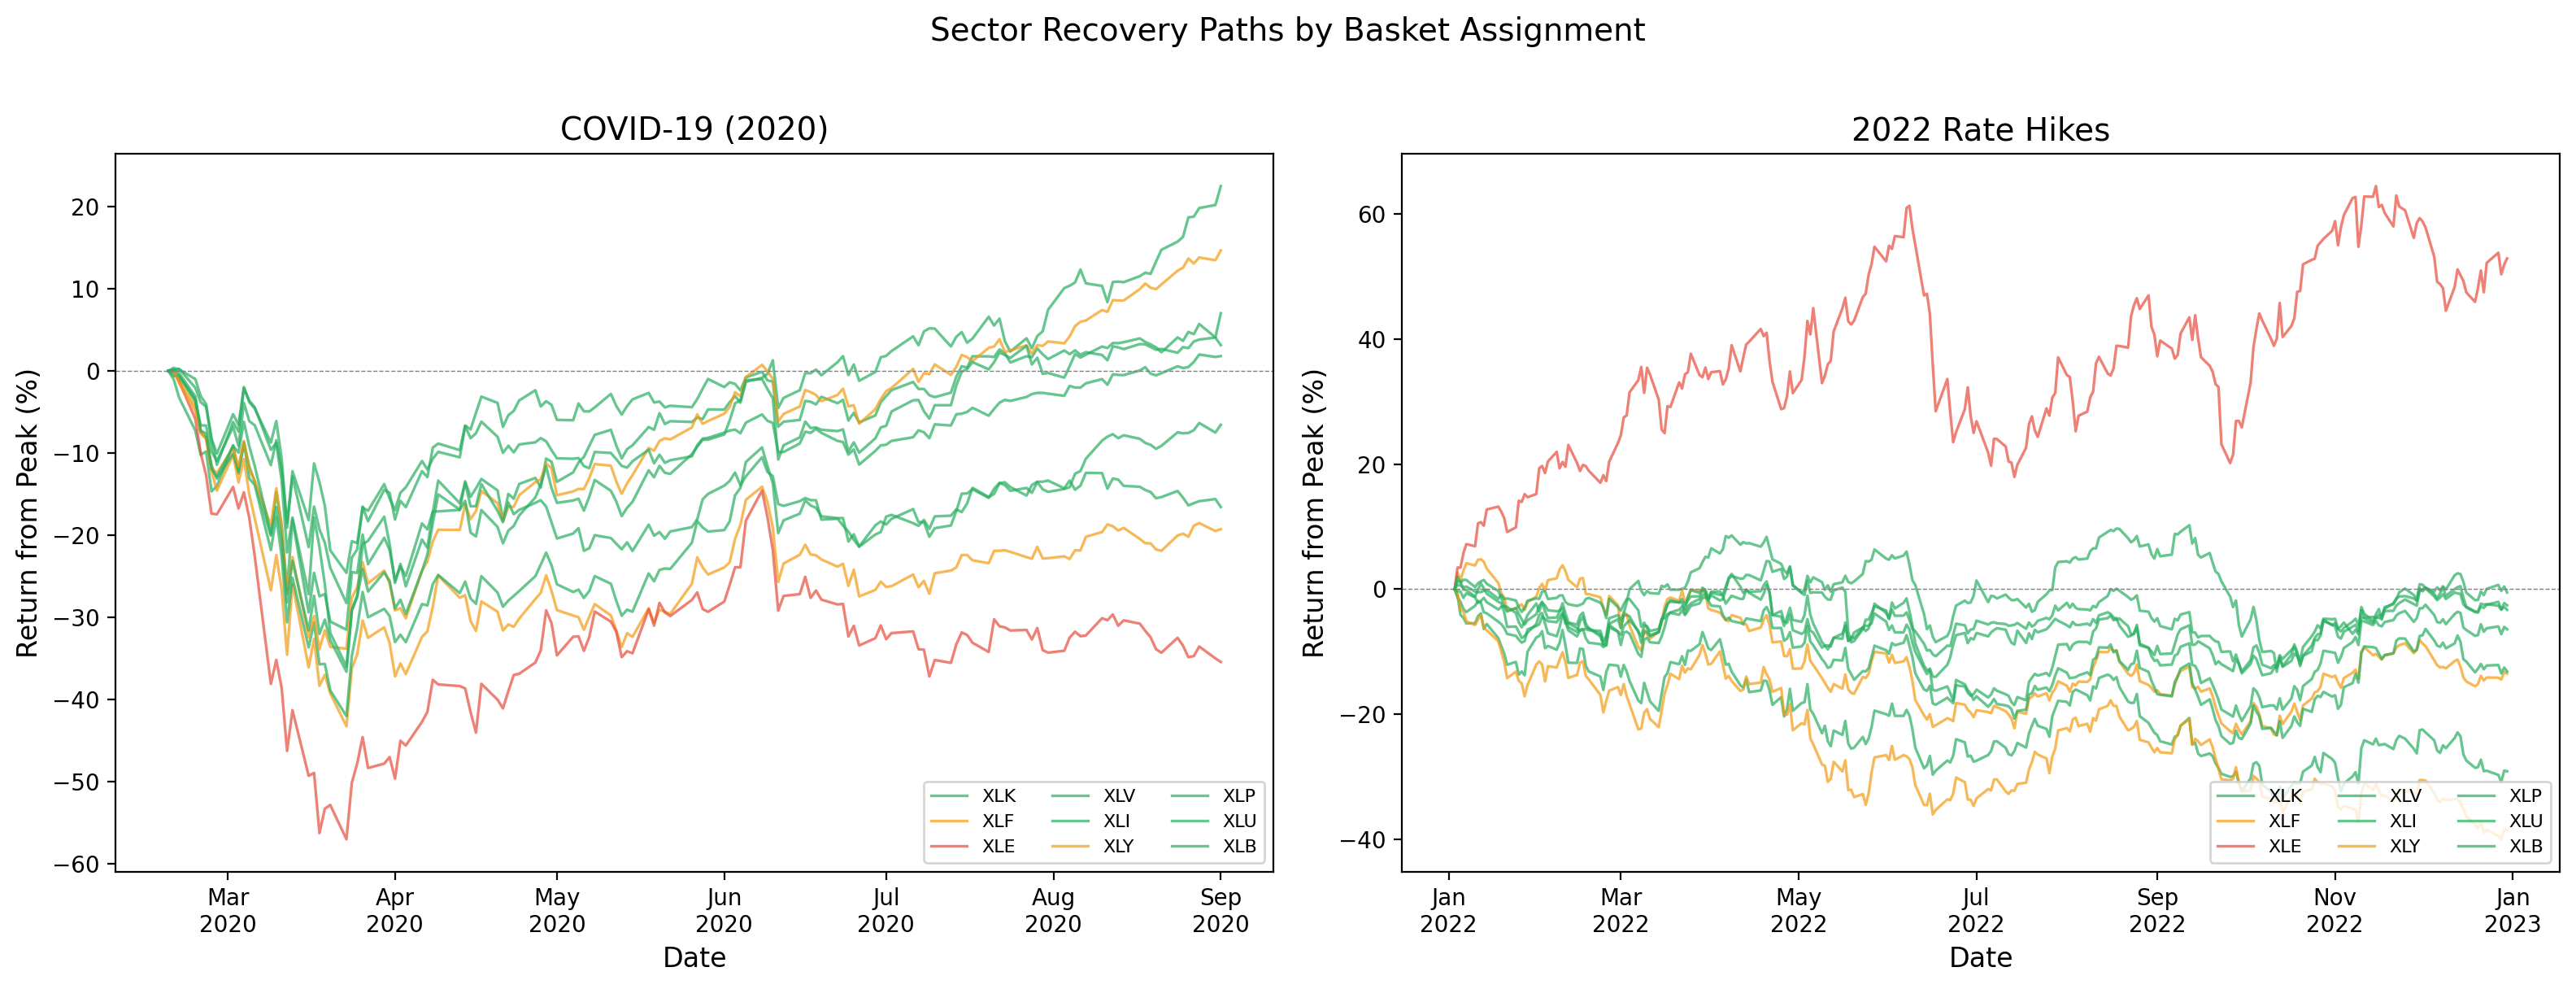
\includegraphics[width=\textwidth]{recovery_analysis.png}
\caption{Sector recovery paths from peak during COVID-19 (left) and
the 2022 rate-hiking cycle (right), colored by basket assignment (red
= Tactical, orange = Avoid, green = Core).  Recovery speed
differences validate the OU half-life classification: Basket~A
sectors recover fastest from the COVID trough, while Basket~B sectors
lag.  During 2022, Energy (XLE, red) exhibits dramatic divergence,
demonstrating regime-dependent sector dynamics.}
\label{fig:recovery}
\end{figure}

% ─── DISCUSSION ──────────────────────────────────────────────────────────────
\section{Discussion}

\subsection{The Normalization Problem}

A key design insight is that portfolio weight normalization can
\emph{negate} regime-responsive behavior.  In the standard approach,
inverse-volatility weights for $N$ assets produce raw sums of
$\sim 20$--$30$.  When stressed assets are de-weighted and the result
is normalized to sum to 1.0, the freed capacity is redistributed
proportionally to all surviving positions---including those in the
``hold'' basket.  This means the portfolio \emph{increases} its
allocation to Core assets during stress, which is the opposite of
risk reduction.  Our approach normalizes base weights to 1.0 before
stress scaling, so that post-scaling sums below 1.0 represent genuine
cash allocation.

\subsection{Detector Scale Invariance}

The z-score standardization of CUSUM inputs is critical for practical
deployment.  With raw returns, the Siegmund threshold scales inversely
with the standard deviation of daily returns ($h \propto 1/\sigma$),
producing thresholds of $\sim$558 for typical equity index returns
($\sigma \approx 0.012$).  Daily accumulator increments of $\sim$0.04
require thousands of consecutive crash days to trigger.  In z-score
space, the threshold is $\sim$6.70 regardless of the return scale,
and a single $-5\%$ day ($z \approx -4.2$) produces a meaningful
signal of 0.55.

\subsection{Limitations}

The framework has several limitations.  First, the annualized turnover
of 4.01$\times$ creates transaction cost drag.  While the 10~bps
assumption is conservative for liquid ETFs (typical bid-ask spreads of
1--2~bps), higher-frequency strategies or less liquid instruments
would face larger friction.  Second, the quarterly recalibration
frequency may be insufficient to capture rapidly evolving market
dynamics; event-driven recalibration could improve responsiveness.
Third, the CUSUM detector's dominance in the post-fix ensemble
suggests that the remaining three detectors may contribute primarily
through ensemble diversity rather than independent predictive power.
Fourth, the backtest spans a single macroeconomic epoch (post-GFC
monetary expansion); performance in structurally different interest
rate environments requires further validation.

\subsection{Robustness}

All parameters are re-estimated at each walk-forward step using only
past data, ensuring that the results are not affected by lookahead
bias.  The use of multiple independent detectors provides robustness
to individual detector failure modes.  The weightless max-of-top-2
consensus---requiring two of four orthogonal detectors to agree---
structurally prevents any single (possibly faulty) detector from moving
the portfolio, with no detector weights to over-fit.  The implicit cash
mechanism provides a natural risk-reduction pathway that does not
depend on correctly predicting the \emph{type} of stress, only its
\emph{presence}.

% ─── CONCLUSION ──────────────────────────────────────────────────────────────
\section{Conclusion}

We have presented a regime-detection framework that fuses four
\emph{orthogonal} stress detectors through a weightless fuzzy consensus
rule for adaptive sector portfolio management. Positioned as a
capital-preservation overlay, the walk-forward validated results hold
maximum drawdown to $-$6.2\% (versus $-$41.7\% for SPY) at a quarter of
the volatility, for a Sharpe of 0.97 versus 0.58. Reported honestly,
simple trend rules achieve higher raw Sharpe on the SPY universe; the
architecture's distinctive value is that it \emph{generalizes}---scoring
Sharpe 1.21 and 1.04 on factor and international universes versus
0.51/0.11 for equal-weight, where an index-tuned rule would not transfer.

The key innovations are: (1)~z-score standardization of CUSUM inputs for
scale-invariant detection; (2)~four orthogonal detector dimensions
(magnitude, structure, participation, tail asymmetry); (3)~a weightless
max-of-top-2 consensus aggregator that requires two detectors to agree,
suppressing single-detector false alarms with no weights to over-fit;
and (4)~implicit cash allocation through sub-unity weight sums rather
than forced normalization.

The framework's value lies not in predicting market direction but in
reliably detecting the \emph{onset} of stress and responding with
genuine risk reduction. During the COVID-19 crash the portfolio moved
sharply to cash within days of the drawdown onset and gradually
re-entered during recovery. This asymmetric response---fast to de-risk,
gradual to re-risk---is the primary driver of the improved risk-adjusted
profile.

Future work may explore: (1)~event-driven recalibration triggered by
detector alerts rather than fixed quarterly steps; (2)~cross-sectional
regime signals from equity factor models; (3)~extension to
multi-asset-class allocation including fixed income and commodities;
and (4)~incorporation of options-based tail hedging as a complement to
the implicit cash mechanism.

% ─── REFERENCES ──────────────────────────────────────────────────────────────
\bibliographystyle{plainnat}

\begin{thebibliography}{20}

\bibitem[Ang and Bekaert(2002)]{ang2002}
A.~Ang and G.~Bekaert.
\newblock International asset allocation with regime shifts.
\newblock \emph{Review of Financial Studies}, 15(4):1137--1187, 2002.

\bibitem[Bollerslev(1986)]{bollerslev1986}
T.~Bollerslev.
\newblock Generalized autoregressive conditional heteroskedasticity.
\newblock \emph{Journal of Econometrics}, 31(3):307--327, 1986.

\bibitem[Brier(1950)]{brier1950}
G.~W. Brier.
\newblock Verification of forecasts expressed in terms of probability.
\newblock \emph{Monthly Weather Review}, 78(1):1--3, 1950.

\bibitem[Engle(1982)]{engle1982}
R.~F. Engle.
\newblock Autoregressive conditional heteroscedasticity with estimates
  of the variance of {United Kingdom} inflation.
\newblock \emph{Econometrica}, 50(4):987--1007, 1982.

\bibitem[Fama and French(2015)]{fama2015}
E.~F. Fama and K.~R. French.
\newblock A five-factor model of expected stock returns.
\newblock \emph{Journal of Financial Economics}, 116(1):1--22, 2015.

\bibitem[Gradojevic and Gen\c{c}ay(2013)]{gradojevic2013}
N.~Gradojevic and R.~Gen\c{c}ay.
\newblock Fuzzy logic, trading uncertainty, and technical trading.
\newblock \emph{Journal of Banking \& Finance}, 37(2):578--586, 2013.

\bibitem[Hamilton(1989)]{hamilton1989}
J.~D. Hamilton.
\newblock A new approach to the economic analysis of nonstationary time
  series and the business cycle.
\newblock \emph{Econometrica}, 57(2):357--384, 1989.

\bibitem[Killick et~al.(2012)]{killick2012}
R.~Killick, P.~Fearnhead, and I.~A. Eckley.
\newblock Optimal detection of changepoints with a linear computational
  cost.
\newblock \emph{Journal of the American Statistical Association},
  107(500):1590--1598, 2012.

\bibitem[Kirby and Ostdiek(2012)]{kirby2012}
C.~Kirby and B.~Ostdiek.
\newblock It's all in the timing: Simple active portfolio strategies
  that outperform na\"ive diversification.
\newblock \emph{Journal of Financial and Quantitative Analysis},
  47(2):437--467, 2012.

\bibitem[Longerstaey and Spencer(1996)]{longerstaey1996}
J.~Longerstaey and M.~Spencer.
\newblock \emph{RiskMetrics Technical Document}.
\newblock J.P.~Morgan/Reuters, 1996.

\bibitem[Nystrup et~al.(2017)]{nystrup2017}
P.~Nystrup, B.~W. Hansen, H.~Madsen, and E.~Lindstr\"{o}m.
\newblock Regime-based versus static asset allocation: Letting the data
  speak.
\newblock \emph{Journal of Risk}, 19(6), 2017.

\bibitem[Page(1954)]{page1954}
E.~S. Page.
\newblock Continuous inspection schemes.
\newblock \emph{Biometrika}, 41(1/2):100--115, 1954.

\bibitem[Siegmund(1985)]{siegmund1985}
D.~Siegmund.
\newblock \emph{Sequential Analysis: Tests and Confidence Intervals}.
\newblock Springer, 1985.

\bibitem[Takagi and Sugeno(1985)]{takagi1985}
T.~Takagi and M.~Sugeno.
\newblock Fuzzy identification of systems and its applications to
  modeling and control.
\newblock \emph{IEEE Transactions on Systems, Man, and Cybernetics},
  (1):116--132, 1985.

\bibitem[Uhlenbeck and Ornstein(1930)]{uhlenbeck1930}
G.~E. Uhlenbeck and L.~S. Ornstein.
\newblock On the theory of the {Brownian} motion.
\newblock \emph{Physical Review}, 36(5):823, 1930.

\end{thebibliography}

\end{document}